\documentclass[]{elsarticle} %review=doublespace preprint=single 5p=2 column
%%% Begin My package additions %%%%%%%%%%%%%%%%%%%
\usepackage[hyphens]{url}

  \journal{An awesome journal} % Sets Journal name


\usepackage{lineno} % add
  \linenumbers % turns line numbering on
\providecommand{\tightlist}{%
  \setlength{\itemsep}{0pt}\setlength{\parskip}{0pt}}

\usepackage{graphicx}
\usepackage{booktabs} % book-quality tables
%%%%%%%%%%%%%%%% end my additions to header

\usepackage[T1]{fontenc}
\usepackage{lmodern}
\usepackage{amssymb,amsmath}
\usepackage{ifxetex,ifluatex}
\usepackage{fixltx2e} % provides \textsubscript
% use upquote if available, for straight quotes in verbatim environments
\IfFileExists{upquote.sty}{\usepackage{upquote}}{}
\ifnum 0\ifxetex 1\fi\ifluatex 1\fi=0 % if pdftex
  \usepackage[utf8]{inputenc}
\else % if luatex or xelatex
  \usepackage{fontspec}
  \ifxetex
    \usepackage{xltxtra,xunicode}
  \fi
  \defaultfontfeatures{Mapping=tex-text,Scale=MatchLowercase}
  \newcommand{\euro}{€}
\fi
% use microtype if available
\IfFileExists{microtype.sty}{\usepackage{microtype}}{}
\bibliographystyle{elsarticle-harv}
\usepackage{longtable}
\usepackage{graphicx}
\ifxetex
  \usepackage[setpagesize=false, % page size defined by xetex
              unicode=false, % unicode breaks when used with xetex
              xetex]{hyperref}
\else
  \usepackage[unicode=true]{hyperref}
\fi
\hypersetup{breaklinks=true,
            bookmarks=true,
            pdfauthor={},
            pdftitle={A comparison of design-based and model-based approaches for spatial data.},
            colorlinks=false,
            urlcolor=blue,
            linkcolor=magenta,
            pdfborder={0 0 0}}
\urlstyle{same}  % don't use monospace font for urls

\setcounter{secnumdepth}{5}
% Pandoc toggle for numbering sections (defaults to be off)

% Pandoc citation processing

% Pandoc header

\usepackage{bm} \usepackage{bbm} \usepackage{color} \DeclareMathOperator{\var}{{var}} \DeclareMathOperator{\cov}{{cov}}

\begin{document}
\begin{frontmatter}

  \title{A comparison of design-based and model-based approaches for spatial
data.}
    \author[USEPA]{In alphabetical order Michael Dumelle\corref{1}}
   \ead{Dumelle.Michael@epa.gov} 
    \author[STLAW]{Matt Higham\corref{1}}
   \ead{mhigham@stlaw.edu} 
    \author[OSU]{Lisa Madsen}
  
    \author[USEPA]{Anthony R. Olsen}
  
    \author[NOAA]{Jay M. Ver Hoef}
  
      \address[USEPA]{United States Environmental Protection Agency, 200 SW 35th St,
Corvallis, Oregon, 97333}
    \address[STLAW]{Saint Lawrence University Department of Math, Computer Science, and
Statistics, 23 Romoda Drive, Canton, New York, 13617}
    \address[OSU]{Oregon State University Department of Statistics, 239 Weniger Hall,
Corvallis, Oregon, 97331}
    \address[NOAA]{Marine Mammal Laboratory, Alaska Fisheries Science Center, National
Oceanic and Atmospheric Administration, Seattle, Washington, 98115}
      \cortext[1]{Corresponding Author}
  
  \begin{abstract}
  This is the abstract.
  \end{abstract}
  
 \end{frontmatter}

\emph{Text based on elsarticle sample manuscript, see
\url{http://www.elsevier.com/author-schemas/latex-instructions\#elsarticle}}

Potential Journals:

\begin{itemize}
\tightlist
\item
  Ecological Applications
\item
  Methods in Ecology and Evolution
\item
  Journal of Applied Ecology
\item
  Environmetrics
\item
  Environmental and Ecological Statistics
\end{itemize}

\hypertarget{sec:introduction}{%
\section{Introduction}\label{sec:introduction}}

There are two general approaches for using data to make statistical
inferences about a population: design-based approaches and model-based
approaches. When data cannot be obtained for all units in a population
(population units), data on a subset of the population units is
collected in a sample. In the design-based approach, inferences about
the underlying population are informed from a probabilistic process in
which population units are selected to be in the sample. Alternatively,
in the model-based approach, inferences are made from specific
assumptions about the underlying process that generated the data. Each
paradigm has a deep historical context (Sterba, 2009) and its own set of
general advantages (Hansen et al., 1983).

Though the design-based and model-based approaches apply to statistical
inference in a broad sense, we focus on comparing these approaches for
spatial data. We define spatial data as variables measured at specific
geographic locations. De Gruijter and Ter Braak (1990) give an early
comparison of design-based and model-based approaches for spatial data,
quashing the belief that design-based approaches could not be used for
spatially correlated data. Thereafter, several comparisons between
design-based and model-based for spatial data have been considered, but
they tend to compare design-based approaches that ignore spatial
locations to model-based approaches (Brus and De Gruijter, 1997; Ver
Hoef, 2002, 2008). Cooper (2006) review the two approaches in an
ecological context before introducing a ``model-assisted'' variance
estimator that combines aspects from each approach. In addition to
Cooper (2006), there has been substantial research and development into
estimators that use both design and model-based principles (see
e.g.~Cicchitelli and Montanari (2012), Chan-Golston et al. (2020) for a
Bayesian approach, and Sterba (2009)). More recent overviews include
Brus (2020) and Wang et al. (2012), but no numerical comparison has been
made between design-based approaches that incorporate spatial locations
and model-based approaches.

The rest of this paper is organized as follows. In Section
\ref{sec:background}, we compare sampling and estimation procedures
between the design-based approach and the model-based approach. In
Section \ref{sec:numstudy}, we use simulated and real data to study the
the behavior of both approaches. And in Section \ref{sec:discussion}, we
end with a discussion and provide directions for future research.

\hypertarget{sec:background}{%
\section{Background}\label{sec:background}}

The design-based and model-based approaches incorporate randomness in
fundamentally different ways. In this section, we describe the role of
randomness and its effects on subsequent inferences. We then discuss
specific inference methods for the design-based and model-based
approaches for spatial data.

\hypertarget{comparing-design-based-vs.-model-based}{%
\subsection{Comparing Design-Based
vs.~Model-Based}\label{comparing-design-based-vs.-model-based}}

The design-based approach assumes the data are fixed. Randomness is
incorporated in the selection of population units according to a
sampling design. A sampling design assigns a positive probability of
inclusion in the sample (inclusion probability) to each population unit.
Some examples of commonly used sampling designs include independent
random sampling (IRS), stratified random sampling, and cluster sampling.
The goal is to use the sampling design and the sampled data to estimate
population parameters like means and totals. These population parameters
are typically assumed to be fixed but unknown.

Treating the data as fixed and incorporating randomness through the
sampling design yields estimators having very few other assumptions.
Confidence intervals for these types of estimators are typically derived
using limiting arguments. Means and totals, for example, are
asymptotically normally distributed by the Central Limit Theorem.
Särndal et al. (2003) and Lohr (2009) provide thorough reviews of the
design-based approach.

The model-based approach assumes the data are a random realization of a
data-generating process. Randomness is often incorporated through
distributional assumptions on this process. Instead of estimating fixed
but unknown parameters (as in the design-based approach), the goal of
model-based inference in the spatial context is often \emph{prediction}
of an unknown quantity. For example, suppose the realized mean of all
population units is the quantity of interest. Instead of
\emph{estimating} a fixed unknown mean, we are \emph{predicting} the
value of the mean, a random variable. We know that if we sampled all
population units, we would have an exact prediction for the mean of our
one realized process, without any uncertainty. But we are typically not
interested in the true, unknown mean of the underlying process.

Assuming the data is a realization of a specific data-generating process
yields predictors that are linked to distributional assumptions. These
distributional assumptions are used to derive prediction intervals. The
distributional assumptions allow the prediction intervals to be more
precise. Cressie (1993) and Schabenberger and Gotway (2017) provide
reviews of model-based approaches for spatial data.

\begin{figure}
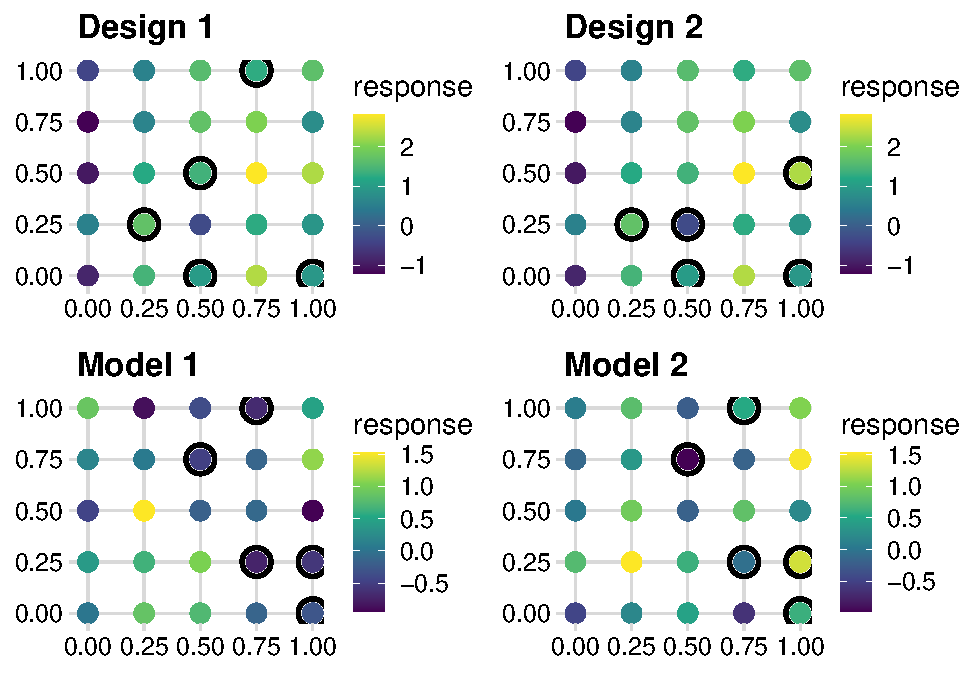
\includegraphics[width=1\linewidth]{SpatialDVM_Manuscript_files/figure-latex/fig1-1} \caption{A comparison of sampling under the design-based and model-based frameworks. In the top row, we have one fixed population, and two random samples. In the bottom row, we have two realizations of the same spatial process sampled at the same locations.}\label{fig:fig1}
\end{figure}

Description of Figure \ref{fig:fig1} goes here.

\hypertarget{spatially-balanced-design-and-analysis}{%
\subsection{Spatially Balanced Design and
Analysis}\label{spatially-balanced-design-and-analysis}}

The design-based approach can use spatial locations to obtain spatially
balanced samples. First we discuss spatial balance with respect to the
population (Stevens Jr and Olsen, 2004). A sample is spatially balanced
with respect to the population if the sampled population units are a
miniature of the population units. A sample is a miniature of the
population if the distribution of the sampled population units mirrors
the density of all population units. Spatial balance with respect to the
population is different than spatial balance with respect to geography.
A sample that is spatially balanced with respect to geography is spread
out in some type of equidistant manner over geographical space and is
not meant to be miniatures of the population. When we refer to spatial
balance henceforth, we mean spatial balance with respect to the
population.

Spatially balanced samples are useful because they tend to yield
estimates that have lower variance than estimates constructed from
sampling designs lacking spatial balance (Barabesi and Franceschi, 2011;
Benedetti et al., 2017; Grafström and Lundström, 2013; Robertson et al.,
2013; Stevens Jr and Olsen, 2004; Wang et al., 2013). To quantify
spatial balance, Stevens Jr and Olsen (2004) proposed loss functions
based on Voroni polygons. The first spatially balanced sampling
algorithm that saw widespread use was the Generalized Random
Tessellation Stratified (Stevens Jr and Olsen, 2004). Since GRTS was
developed, several other spatially balanced sampling algorithms have
emerged, including the Local Pivotal Method (Grafström et al., 2012;
Grafström and Matei, 2018), Spatially Correlated Poisson Sampling
(Grafström, 2012), Balanced Acceptance Sampling (Robertson et al.,
2013), Within-Sample-Distance (Benedetti and Piersimoni, 2017), and
Halton Iterative Partitioning (Robertson et al., 2018). We focus on the
Generalized Random Tessellation Stratified (GRTS) algorithm to select
spatially balanced sampling because it has several attractive properties
detailed by Stevens Jr and Olsen (2004) and Dumelle et al. (2021).

The GRTS algorithm is used to sample from finite and infinite
populations and works by utilizing a mapping between two-dimensional and
one-dimensional space. The population units in two-dimensional space are
divided into cells using a hierarchical index. Population units are then
mapped to a one-dimensional line via the hierarchical indexing. The line
length of each population unit equals its inclusion probability. A
systematic sample is conducted on the line and these samples are linked
to a population unit in two-dimensional space, which results in the
desired sample. Stevens Jr and Olsen (2004) provide and Dumelle et al.
(2021) provide further details.

After collecting a sample using the GRTS algorithm, the data are used to
estimate population parameters. The Horvitz-Thompson estimator (Horvitz
and Thompson, 1952) yields unbiased estimates of population means and
totals. For example, if \(\tau\) is a population total, then the
Horvitz-Thompson estimator of \(\tau\) (denoted by \(\hat{\tau}_{ht}\)),
is given by \begin{align}\label{eq:ht}
  \hat{\tau}_{ht} = \sum_{i = 1}^n Z_i \pi_i^{-1},
\end{align} where \(Z_i\) and \(\pi_i\) are the observed value and
inclusion probability of the \(i\)th population unit selected in the
sample. A similar formula exists for estimating the mean, \(\mu\).
Horvitz and Thompson (1952) and Sen (1953) provide variance estimators
for \(\hat{\tau}_{ht}\), but they have two drawbacks. First, they rely
on calculating \(\pi_{ij}\), the probability that population unit \(i\)
and population unit \(j\) are included in the sample, and this can be
very difficult to calculate. Second, they ignore the spatial locations
of the population units. To address these drawbacks, Stevens Jr and
Olsen (2003) proposed a local neighborhood variance estimator. The local
neighborhood variance estimator does not rely on \(\pi_{ij}\), and it
incorporates spatial locations by assigning higher weights to nearby
observations. Stevens Jr and Olsen (2003) show this variance estimators
tends to reduce the estimated standard error of \(\hat{\tau}\), yielding
narrower confidence confidence intervals for \(\tau\).

\hypertarget{finite-population-block-kriging}{%
\subsection{Finite Population Block
Kriging}\label{finite-population-block-kriging}}

Finite Population Block Kriging (FPBK) is a model-based approach that
expands the geostatistical Kriging framework to the finite population
setting (Ver Hoef, 2008). Instead of basing inference off of a specific
sampling design, we assume the data are generated by a spatial process.
Ver Hoef (2008) gives details on the theory of FPBK, but some of the
basic principles are summarized below. Let
\(\mathbf{z} \equiv \{\text{z}(s_1), \text{z}(s_2), . . . , \text{z}(s_N) \}\)
be a response variable that can be measured at the \(N\) population
units and is represented as an \(N \times 1\) vector. Suppose we want to
predict some linear function of the response variable,
\(f(\mathbf{z}) = \mathbf{b}^\prime \mathbf{z}\), where \(\mathbf{b}\)
is a \(1 \times N\) vector of weights. For example, if we want to
predict the population total across all population units, then we would
use a vector of 1's for the weights.

Typically, however, we only have a sample of the \(N\) population units.
Denoting quantities that are part of the sampled population units with a
subscript \emph{s} and quantities that are part of the unsampled
population units with a subscript \emph{u},

\begin{equation}
\begin{pmatrix} \label{equation:Zmarginal}
    \mathbf{z}_s      \\
    \mathbf{z}_u
\end{pmatrix}
=
\begin{pmatrix}
  \mathbf{X}_s    \\
  \mathbf{X}_u
\end{pmatrix}
\bm{\beta} +
\begin{pmatrix}
\bm{\delta}_s    \\
\bm{\delta}_u
\end{pmatrix},
\end{equation} where \(\mathbf{X}_s\) and \(\mathbf{X}_u\) are the
design matrices for the sampled and unsampled population units,
respectively; \(\beta\) is the parameter vector of fixed effects; and
\(\bm{\delta}_s\) and \(\bm{\delta}_u\) are random errors for the
sampled and unsampled population units, respectively. Denoting
\(\bm{\delta} \equiv [\bm{\delta}_s \,\, \bm{\delta}_u]'\), we assume
the expectation of \(\bm{\delta}\) equals \(\mathbf{0}\).

We also typically assume that there is spatial correlation in
\(\bm{\delta}\), which can be modeled using a covariance function. It is
common to assume the covariance function is second-order stationary and
isotropic (Cressie, 1993), and that the spatial covariance decreases as
the separation between population units increases. Many spatial
covariance functions exist, but the primary function we use throughout
the simulations and applications in this manuscript is the exponential
covariance function: the \(i,j^{th}\) entry for
\(\mathop{\mathrm{{cov}}}(\bm{\delta})\) is \mbox{}
\begin{align}\label{equation:expcov}
\mathop{\mathrm{{cov}}}(\delta_i, \delta_j) = \theta_1\exp(-3h_{i,j}/\theta_2) + \theta_3\mathbbm{1}\{\mathbf{h}_{i,j} = 0\}, 
\end{align} where \(h_{i,j}\) is the distance between population units
\(i\) and \(j\), and \(\bm{\theta}\) is a vector of spatial covariance
parameters of the partial sill \(\theta_1\), the range \(\theta_2\), and
the nugget \(\theta_3\), and \(\mathbbm{1}\) is an indicator function.
However, any spatial covariance function could be used in the place of
the exponential, including functions that allow for non-stationarity or
anisotropy (Chiles and Delfiner, 1999, pp. 80--93).

With the above model formulation, the Best Linear Unbiased Predictor
(BLUP) for \(f(\mathbf{b}'\mathbf{z})\) and its prediction variance can
be computed. While details of the derivation are in (Ver Hoef, 2008), we
note here that the predictor and its variance are both moment-based.

We note that we only use FPBK in this paper in order to focus more on
comparing the design-based and model-based approaches. However,
k-nearest-neighbors (Fix and Hodges, 1951; Ver Hoef and Temesgen, 2013),
random forest (Breiman, 2001), Bayesian models (Chan-Golston et al.,
2020), among others, can also be used to obtain predictions for a mean
or total from spatially correlated responses in a finite population
setting.

\hypertarget{sec:numstudy}{%
\section{Numerical Study}\label{sec:numstudy}}

There were several variables to alter in the simulations, and the names
of the scenarios in future plots mirror these variables

\begin{itemize}
\tightlist
\item
  correlation type: dependent errors or independent errors
\item
  error type:

  \begin{itemize}
  \tightlist
  \item
    normal: mean 0, variance 2
  \item
    lognormal: log scale mean 0, log scale variance 2 (total variance
    47)
  \item
    lognormalbig: log scale mean 0, log scale variance 4 (total variance
    2,926)
  \end{itemize}
\item
  sample sizes: \(n = 10, 50, 150; N = 900\)
\item
  layout: gridded vs random population locations
\end{itemize}

So for example, the \texttt{inderror.normal.n50.randloc} is the
simulation having independent random errors that are normal, a sample
size of 50, and random population locations.

There were 2000 trials for each simulation. The original response
(before exponentiating if applicable) for the dependent error cases was
normally distributed with an exponential covariance function with
partial sill of 0.9, effective range of \(\sqrt{2}\), and a nugget of
0.1. For the independent error cases, the partial sill was 0 and the
nugget was 1.

In each simulation, a GRTS sample and an IRS sample were selected. Then
for the GRTS sample, the design-based approach using the local
neighborhood variance (Design GRTS) and a model-based approach were
applied (Model GRTS). Then for the IRS sample, the design-based approach
using the simple random sample variance (Design IRS) and a model-based
approach were applied (Model IRS).

The GRTS algorithm and the local neighborhood variance estimator are
available in the \textbf{\textsf{R}} package \texttt{spsurvey} (Dumelle
et al., 2021). FPBK can be readily performed in \texttt{R} with the
\texttt{sptotal} package (Higham et al., 2020). We use \texttt{sptotal}
for both the simulation analysis and the application, estimating
parameters with Restricted Maximum Likelihood (REML).

Major Points from August 3 Simulations:

\begin{enumerate}
\def\labelenumi{\arabic{enumi}.}
\tightlist
\item
  In most of the dependent error simulation settings, either all four
  approahces (IRS-Design, IRS-Model, GRTS-Design, and GRTS-Model)
  perform equally or GRTS-Design and GRTS-Model outperform IRS-Design
  and IRS-Model. Exceptions to this are a couple of the settings with
  very small sample sizes (n = 10), in which the IRS does better than
  GRTS. In the independent error settings, it usually doesn't matter
  much which approach is used, which makes sense.
\end{enumerate}

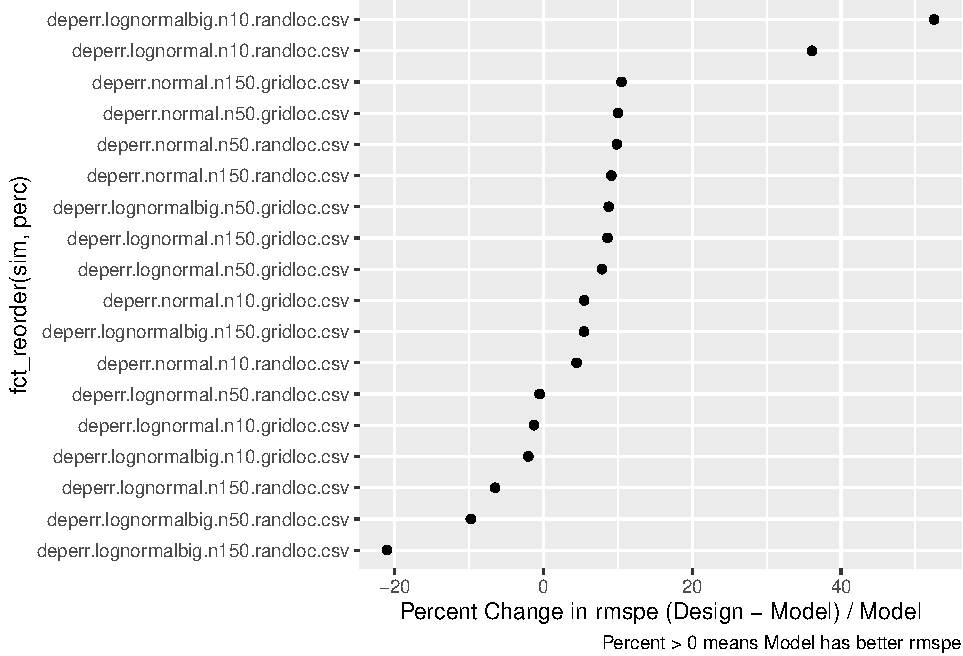
\includegraphics{SpatialDVM_Manuscript_files/figure-latex/unnamed-chunk-4-1.pdf}

\begin{enumerate}
\def\labelenumi{\arabic{enumi}.}
\setcounter{enumi}{1}
\tightlist
\item
  We will now focus in a bit more on comparing Design-GRTS to
  Model-GRTS, the two best approaches for any reasonable sample size. In
  the independent error settings, the two approaches perform very
  similarly, so those results are omitted in the following graph. In the
  dependent error settings, using rmspe as the performance criterion,
  Model-GRTS outperforms Design-GRTS in 12 of the 18 settings, the two
  approaches perform very similarly in 3 settings, and Design-GRTS
  outperforms Model-GRTS in 3 settings.
\end{enumerate}

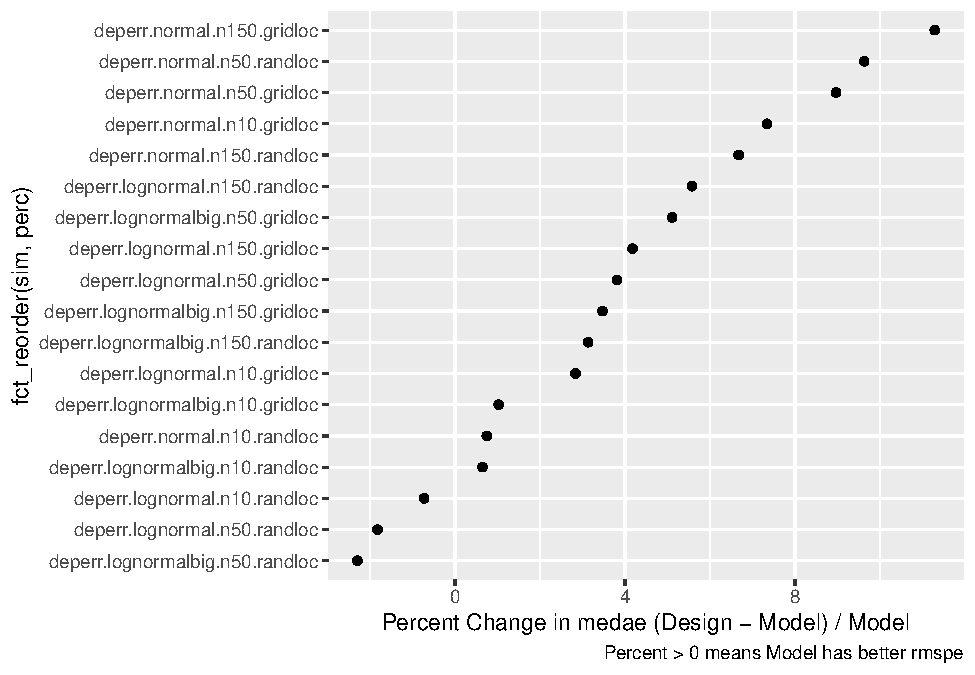
\includegraphics{SpatialDVM_Manuscript_files/figure-latex/unnamed-chunk-5-1.pdf}
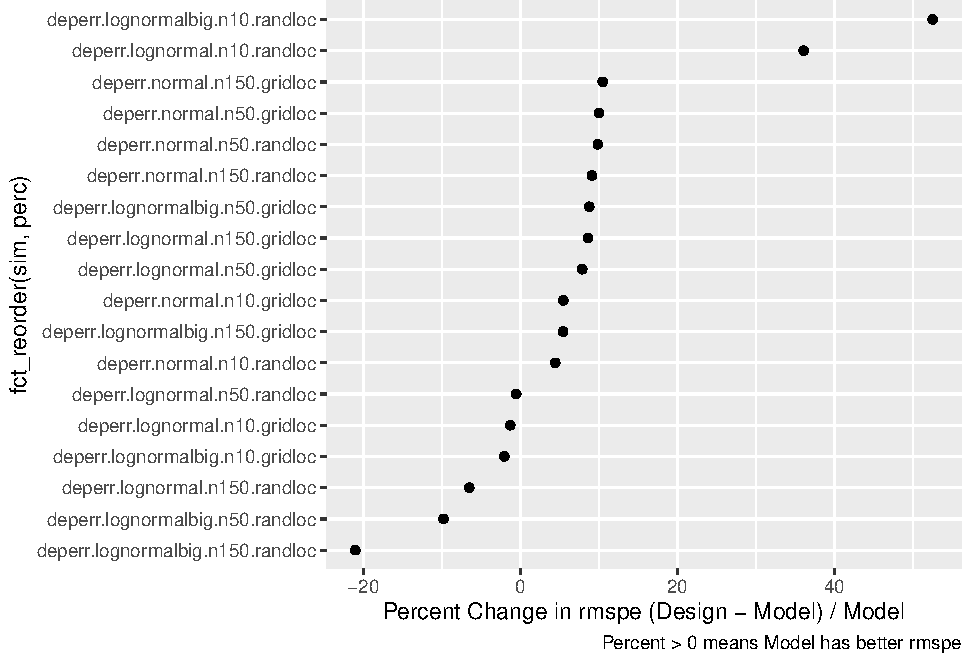
\includegraphics{SpatialDVM_Manuscript_files/figure-latex/unnamed-chunk-5-2.pdf}

\begin{enumerate}
\def\labelenumi{\arabic{enumi}.}
\setcounter{enumi}{2}
\tightlist
\item
  Focusing in on the three settings where Design-GRTS outperforms
  Model-GRTS, we see that, in two of the settings, the log-normal
  response has a large variance, corresponding to a large right-skew
  after exponentiation. All three settings have sites in random
  locations. However, in only one of these settings would we recommend
  actually using Design-GRTS. In the other two settings, the data are
  sufficiently skewed that a practitioner should not use either
  approach, though it is ``safer'' to use Design-GRTS.
\end{enumerate}

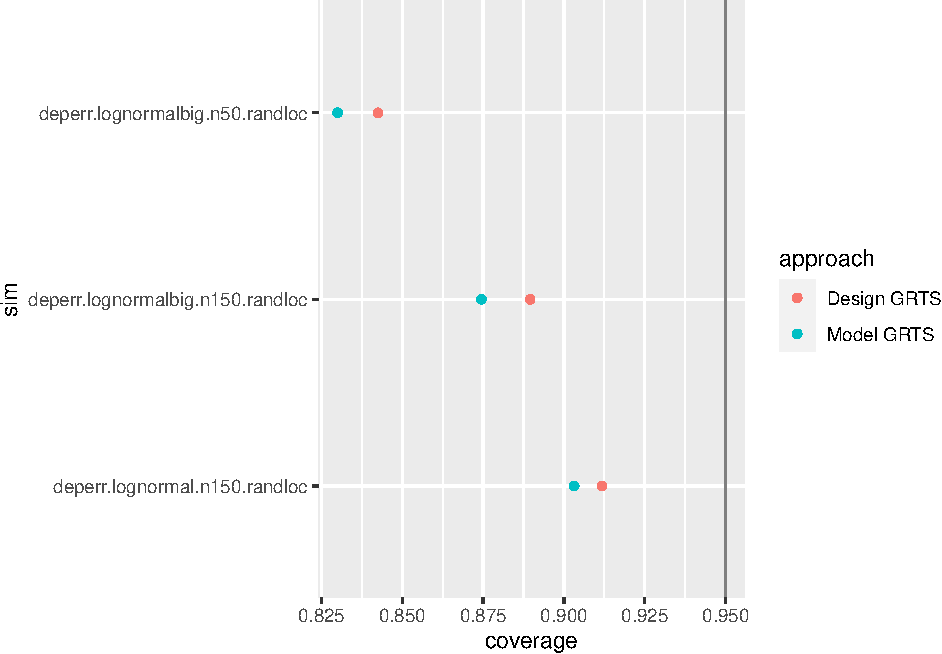
\includegraphics{SpatialDVM_Manuscript_files/figure-latex/unnamed-chunk-6-1.pdf}

\begin{enumerate}
\def\labelenumi{\arabic{enumi}.}
\setcounter{enumi}{3}
\tightlist
\item
  Coverage
\end{enumerate}

For Gaussian errors, coverage for all approaches tended to be near 0.95.
There was less between-approach deviation in coverages for random
locations compared to grid locations. Generally, the larger the skew,
the worse the coverage,and the larger the sample size, the better the
coverage. Design GRTS (local neighborhood variance) tended to slightly
undercover, a result Tony was familiar with.

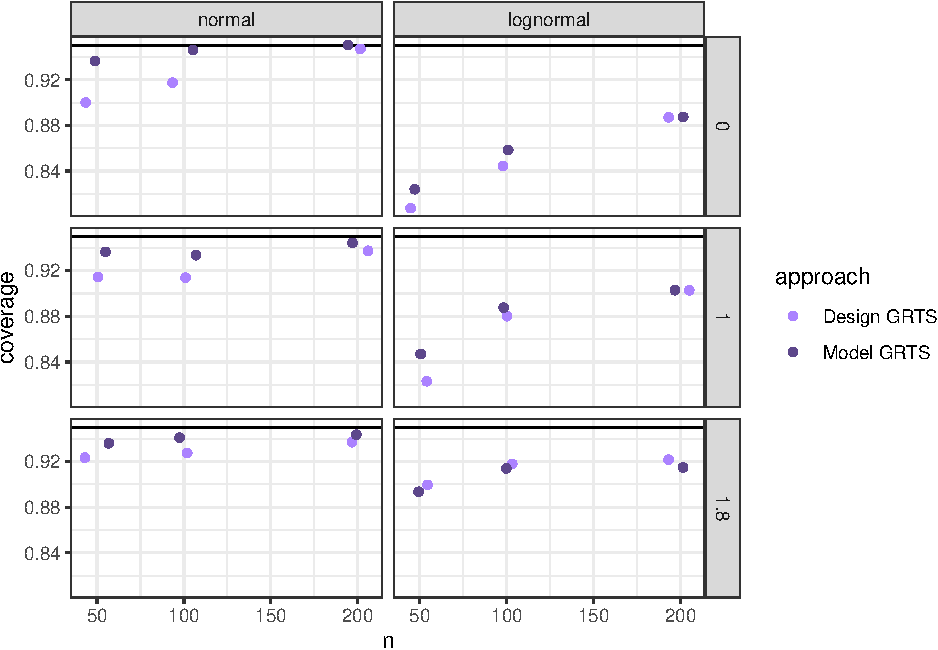
\includegraphics{SpatialDVM_Manuscript_files/figure-latex/unnamed-chunk-7-1.pdf}

\begin{enumerate}
\def\labelenumi{\arabic{enumi}.}
\setcounter{enumi}{4}
\tightlist
\item
  Take-home messages
\end{enumerate}

\begin{itemize}
\tightlist
\item
  In terms of rmspe, a model-based analysis on a GRTS design yields an
  rmspe similar to or lower than a design-based analysis on a GRTS
  design, as long as the response variable is not ``too skewed.''
\item
  If the response variable is very skewed, then neither analysis is
  appropriate, but, the design-based analysis is better.
\item
  a spatially balanced GRTS sample outperforms IRS in nearly all
  dependent error settings, as expected.
\item
  methods that use spatial correlation generally perform better on
  random location points than they do on gridded points. This makes some
  intuitive sense because (1) on average, the minimum distance between
  an unobserved point and its nearest observed neighbor should be lower
  for random points and (2) the span of the study area is maximized for
  a grid based on the way that we set up the simulations (with the
  random points being drawn as uniform random variables within the
  boundary of the grid).
\item
  comparison of Design-GRTS and Model-GRTS between two settings with
  different locations of points, but otherwise the same simulation
  parameters, should really be done on the same surface realization. One
  very strange realized response vector could drastically alter the
  results, especially on the exponentiated log data. In the same way
  that we compare the four approaches on the same realized data, we
  should also try to do the same with the locations, if they are of
  interest. (The realized mean won't be exactly the same but should be
  close).
\end{itemize}

\hypertarget{application}{%
\section{Application}\label{application}}

The Environmental Protection Agency (EPA), states, and tribes
periodically conduct National Aquatic Research Surveys (NARS) in the
United States to assess the water quality of various bodies of water. We
will use the 2012 National Lakes Assessment (NLA), which measures
various aspects of lake health and quality in lakes in the contiguous
United States, to obtain an interval for mean mercury concentration.
Although all lakes in the survey were measured in 2012, there may not
always be enough time or money to do so. Therefore, we will explore
whether or not we can still obtain a relatively precise estimate for the
realized mean mercury concentration if we only take a sample of 100 of
the 986 lakes.

\begin{figure}
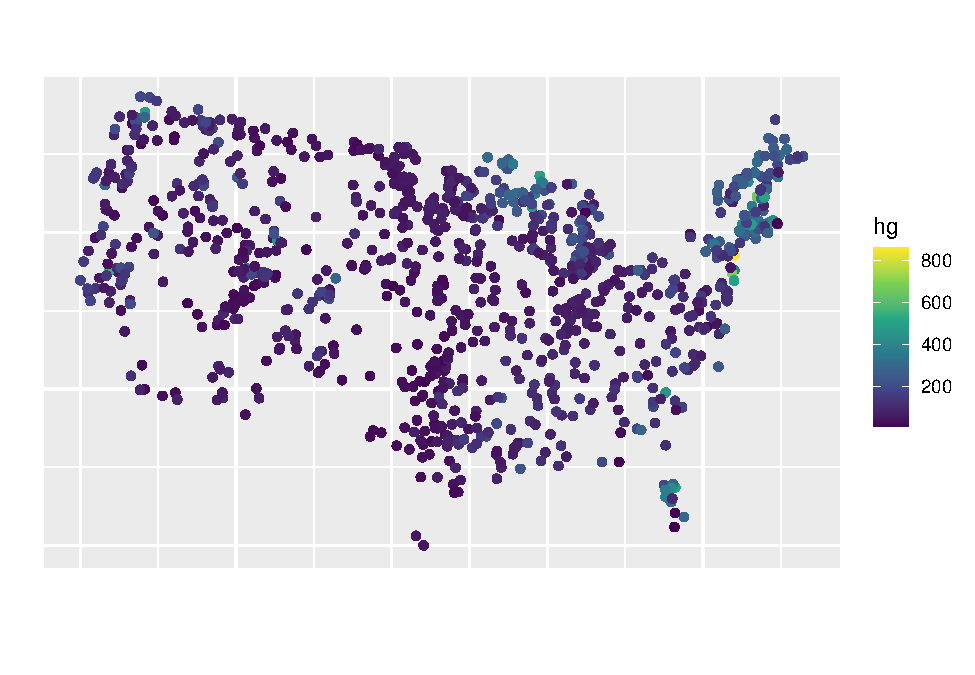
\includegraphics[width=1\linewidth]{SpatialDVM_Manuscript_files/figure-latex/figdata-1} \caption{Population distribution of mercury concentration for 986 lakes in the contiguous United States. Thirty-five lakes were dropped from the analysis because they were missing mercury concentration.}\label{fig:figdata}
\end{figure}

Figure \ref{fig:figdata} shows that mercury concentration is
right-skewed, with most lakes having a low value of mercury
concentration but a few having a much higher concentration. Mercury
concentration exhibits some spatial correlation, with high mercury
concentrations in lakes in the northeast and north central United
States. Because we are considering these lakes to be our entire
population, we know that the realized mean mercury concentration is
103.03 ng / g.

\begin{longtable}[]{@{}lrrrrr@{}}
\caption{\label{tab:appliedtab} Table XXX. Application of design-based
and model-based approaches to the NLA data set on mercury
concentration.}\tabularnewline
\toprule
Approach & Realized Mean & Estimate & SE & 95\% LB & 95\%
UB\tabularnewline
\midrule
\endfirsthead
\toprule
Approach & Realized Mean & Estimate & SE & 95\% LB & 95\%
UB\tabularnewline
\midrule
\endhead
Design IRS & 103.2 & 112.7 & 8.8 & 95.4 & 129.9\tabularnewline
Model IRS & 103.2 & 110.5 & 7.9 & 95.0 & 125.9\tabularnewline
Design GRTS & 103.2 & 101.8 & 6.1 & 89.8 & 113.7\tabularnewline
Model GRTS & 103.2 & 102.3 & 5.9 & 90.8 & 113.9\tabularnewline
\bottomrule
\end{longtable}

Table \ref{tab:appliedtab} shows the application of a design-based
analysis on an IRS, a model-based analysis on an IRS, a design-based
analysis on a GRTS sample, and a model-based analysis on a GRTS sample.
We see that, for all four analyses, the true realized mean mercury
concentration is within the bounds of the 95\% intervals. However, we
should not generalize the results of this particular realization to any
other data set or even to other potential samples of this data set.

But, we do note a couple of patterns. The design-based IRS analysis
shows the largest standard error: a likely reason is that this is the
only approach that does not use the spatial correlation in mercury
concentration across the contiguous United States. We also see that, for
the samples drawn, the both analyses with the GRTS sampling design have
a lower standard error than the analyses with the IRS sampling design.
We would expect this to be the case for most samples because mercury
concentration exhibits spatial correlation so a spatially balanced
sample should usually yield a lower standard error. If it is acceptable
to have an interval for mean mercury concentration of about 25 ng / g
and if we ignore the other variables that the EPA collects information
on in these NLA surveys, then the EPA could consider sampling just 50
lakes to save time and money.

\hypertarget{sec:discussion}{%
\section{Discussion}\label{sec:discussion}}

\begin{itemize}
\item
  Pros of Design-Based (items we are not exploring): computationally
  efficient, few assumptions, more naturally handles binary data,
\item
  Pros of Model-Based (items we are not exploring): covariate inference,
  more efficient small-area estimation, model selection?, estimated
  spatial parameters to better understand spatial structure,
  site-by-site predictions/prediction map
\end{itemize}

\hypertarget{references}{%
\section*{References}\label{references}}
\addcontentsline{toc}{section}{References}

\hypertarget{refs}{}
\leavevmode\hypertarget{ref-barabesi2011sampling}{}%
Barabesi, L., Franceschi, S., 2011. Sampling properties of spatial total
estimators under tessellation stratified designs. Environmetrics 22,
271--278.

\leavevmode\hypertarget{ref-benedetti2017spatially}{}%
Benedetti, R., Piersimoni, F., 2017. A spatially balanced design with
probability function proportional to the within sample distance.
Biometrical Journal 59, 1067--1084.

\leavevmode\hypertarget{ref-benedetti2017spatiallyreview}{}%
Benedetti, R., Piersimoni, F., Postiglione, P., 2017. Spatially balanced
sampling: A review and a reappraisal. International Statistical Review
85, 439--454.

\leavevmode\hypertarget{ref-breiman2001random}{}%
Breiman, L., 2001. Random forests. Machine learning 45, 5--32.

\leavevmode\hypertarget{ref-brus1997random}{}%
Brus, D., De Gruijter, J., 1997. Random sampling or geostatistical
modelling? Choosing between design-based and model-based sampling
strategies for soil (with discussion). Geoderma 80, 1--44.

\leavevmode\hypertarget{ref-brus2020statistical}{}%
Brus, D.J., 2020. Statistical approaches for spatial sample survey:
Persistent misconceptions and new developments. European Journal of Soil
Science.

\leavevmode\hypertarget{ref-chan2020bayesian}{}%
Chan-Golston, A.M., Banerjee, S., Handcock, M.S., 2020. Bayesian
inference for finite populations under spatial process settings.
Environmetrics 31, e2606.

\leavevmode\hypertarget{ref-chiles1999geostatistics}{}%
Chiles, J.-P., Delfiner, P., 1999. Geostatistics: Modeling Spatial
Uncertainty. John Wiley \& Sons, New York.

\leavevmode\hypertarget{ref-cicchitelli2012model}{}%
Cicchitelli, G., Montanari, G.E., 2012. Model-assisted estimation of a
spatial population mean. International Statistical Review 80, 111--126.

\leavevmode\hypertarget{ref-cooper2006sampling}{}%
Cooper, C., 2006. Sampling and variance estimation on continuous
domains. Environmetrics: The official journal of the International
Environmetrics Society 17, 539--553.

\leavevmode\hypertarget{ref-cressie1993statistics}{}%
Cressie, N., 1993. Statistics for spatial data. John Wiley \& Sons.

\leavevmode\hypertarget{ref-de1990model}{}%
De Gruijter, J., Ter Braak, C., 1990. Model-free estimation from spatial
samples: A reappraisal of classical sampling theory. Mathematical
geology 22, 407--415.

\leavevmode\hypertarget{ref-dumelle2021spsurvey}{}%
Dumelle, M., Olsen, A.R., Kincaid, T., Weber, M., 2021. Selecting and
analyzing spatial probability samples in r using spsurvey. Manuscript
Submitted for Publication.

\leavevmode\hypertarget{ref-fix1951discriminatory}{}%
Fix, E., Hodges, J.L., 1951. Discriminatory analysis, nonparametric
discrimination: Consistency properties. USAF School of Aviation
Medicine.

\leavevmode\hypertarget{ref-grafstrom2012spatiallypoisson}{}%
Grafström, A., 2012. Spatially correlated poisson sampling. Journal of
Statistical Planning and Inference 142, 139--147.

\leavevmode\hypertarget{ref-grafstrom2013well}{}%
Grafström, A., Lundström, N.L., 2013. Why well spread probability
samples are balanced. Open Journal of Statistics 3, 36--41.

\leavevmode\hypertarget{ref-grafstrom2012spatially}{}%
Grafström, A., Lundström, N.L., Schelin, L., 2012. Spatially balanced
sampling through the pivotal method. Biometrics 68, 514--520.

\leavevmode\hypertarget{ref-grafstrom2018spatially}{}%
Grafström, A., Matei, A., 2018. Spatially balanced sampling of
continuous populations. Scandinavian Journal of Statistics 45, 792--805.

\leavevmode\hypertarget{ref-hansen1983evaluation}{}%
Hansen, M.H., Madow, W.G., Tepping, B.J., 1983. An evaluation of
model-dependent and probability-sampling inferences in sample surveys.
Journal of the American Statistical Association 78, 776--793.

\leavevmode\hypertarget{ref-higham2020sptotal}{}%
Higham, M., Ver Hoef, J., Bryce, F., 2020. Sptotal: Predicting totals
and weighted sums from spatial data.

\leavevmode\hypertarget{ref-horvitz1952generalization}{}%
Horvitz, D.G., Thompson, D.J., 1952. A generalization of sampling
without replacement from a finite universe. Journal of the American
statistical Association 47, 663--685.

\leavevmode\hypertarget{ref-lohr2009sampling}{}%
Lohr, S.L., 2009. Sampling: Design and analysis. Nelson Education.

\leavevmode\hypertarget{ref-robertson2013bas}{}%
Robertson, B., Brown, J., McDonald, T., Jaksons, P., 2013. BAS: Balanced
acceptance sampling of natural resources. Biometrics 69, 776--784.

\leavevmode\hypertarget{ref-robertson2018halton}{}%
Robertson, B., McDonald, T., Price, C., Brown, J., 2018. Halton
iterative partitioning: Spatially balanced sampling via partitioning.
Environmental and Ecological Statistics 25, 305--323.

\leavevmode\hypertarget{ref-sarndal2003model}{}%
Särndal, C.-E., Swensson, B., Wretman, J., 2003. Model assisted survey
sampling. Springer Science \& Business Media.

\leavevmode\hypertarget{ref-schabenberger2017statistical}{}%
Schabenberger, O., Gotway, C.A., 2017. Statistical methods for spatial
data analysis. CRC press.

\leavevmode\hypertarget{ref-sen1953estimate}{}%
Sen, A.R., 1953. On the estimate of the variance in sampling with
varying probabilities. Journal of the Indian Society of Agricultural
Statistics 5, 127.

\leavevmode\hypertarget{ref-sterba2009alternative}{}%
Sterba, S.K., 2009. Alternative model-based and design-based frameworks
for inference from samples to populations: From polarization to
integration. Multivariate behavioral research 44, 711--740.

\leavevmode\hypertarget{ref-stevens2003variance}{}%
Stevens Jr, D.L., Olsen, A.R., 2003. Variance estimation for spatially
balanced samples of environmental resources. Environmetrics 14,
593--610.

\leavevmode\hypertarget{ref-stevens2004spatially}{}%
Stevens Jr, D.L., Olsen, A.R., 2004. Spatially balanced sampling of
natural resources. Journal of the american Statistical association 99,
262--278.

\leavevmode\hypertarget{ref-verhoef2002sampling}{}%
Ver Hoef, J., 2002. Sampling and geostatistics for spatial data.
Ecoscience 9, 152--161.

\leavevmode\hypertarget{ref-verhoef2008spatial}{}%
Ver Hoef, J.M., 2008. Spatial methods for plot-based sampling of
wildlife populations. Environmental and Ecological Statistics 15, 3--13.

\leavevmode\hypertarget{ref-ver2013comparison}{}%
Ver Hoef, J.M., Temesgen, H., 2013. A comparison of the spatial linear
model to nearest neighbor (k-nn) methods for forestry applications. PloS
one 8, e59129.

\leavevmode\hypertarget{ref-wang2013design}{}%
Wang, J.-F., Jiang, C.-S., Hu, M.-G., Cao, Z.-D., Guo, Y.-S., Li, L.-F.,
Liu, T.-J., Meng, B., 2013. Design-based spatial sampling: Theory and
implementation. Environmental modelling \& software 40, 280--288.

\leavevmode\hypertarget{ref-wang2012review}{}%
Wang, J.-F., Stein, A., Gao, B.-B., Ge, Y., 2012. A review of spatial
sampling. Spatial Statistics 2, 1--14.


\end{document}


